% Complete Section 7.6, original PDF 100-101 / printed 90-91.
% block: whitney-forms-de-rham-heading page:100 type:section
\subsection{\BT{The Whitney forms $\mathcal P_1^-\Lambda^k$ and de Rham's theorem}{Whitney 形式 $\mathcal P_1^-\Lambda^k$ 与 de Rham 定理}}\label{sec:whitney-forms-de-rham}

% block: whitney-forms-geometric-dofs page:100 type:ordinary-paragraph
\BT{The lowest degree trimmed polynomial finite element space $\mathcal P_1^-\Lambda^k(\mathcal T_h)$ is a subspace of $H\Lambda^k(\Omega)$. Its elements are called the \emph{Whitney $k$-forms}. Its shape functions $\mathcal P_1^-\Lambda^k=\mathcal P_0\Lambda^k+\kappa\mathcal P_0\Lambda^{k+1}$ form a subspace of the complete space $\mathcal P_1\Lambda^k$ of linear polynomial $k$-forms (a proper subspace if $k>0$). Figure~\ref{fig:whitney-form-dofs} shows element diagrams representing the four spaces $\mathcal P_1^-\Lambda^k$, $0\leq k\leq3$, in three dimensions. Each element diagram shows a single simplex with a symbol placed on a face to mark each DOF occuring there. Notice that the DOFs of the Whitney forms are highly geometric: for the Whitney $k$-forms, there is precisely one DOF on each $k$-dimensional subsimplex---namely, the integral of the trace over the faces---and none on the faces of other dimensions. In fact, these spaces appeared in the book \BookCite{70} of Hassler Whitney in 1957, independently of finite elements.}{最低次修剪多项式有限元空间 $\mathcal P_1^-\Lambda^k(\mathcal T_h)$ 是 $H\Lambda^k(\Omega)$ 的子空间. 它的元素称为\emph{Whitney $k$-形式}. 其形函数 $\mathcal P_1^-\Lambda^k=\mathcal P_0\Lambda^k+\kappa\mathcal P_0\Lambda^{k+1}$ 构成线性多项式 $k$-形式的完全空间 $\mathcal P_1\Lambda^k$ 的子空间 (当 $k>0$ 时为真子空间). Figure~\ref{fig:whitney-form-dofs} 展示了表示三维中四个空间 $\mathcal P_1^-\Lambda^k$, $0\leq k\leq3$ 的单元图. 每幅单元图画出一个单纯形, 在面上放置符号, 标明该面上的各个自由度. 注意, Whitney 形式的自由度具有很强的几何性: 对 Whitney $k$-形式, 每个 $k$ 维子单纯形上恰有一个自由度, 即迹在该面上的积分, 而其他维数的面上没有自由度. 事实上, 这些空间独立于有限元, 已在 Hassler Whitney 于 1957 年出版的著作 \BookCite{70} 中出现.}

% block: whitney-form-complex pages:100,101 type:ordinary-paragraph
\BT{As we have seen, the Whitney forms assemble to form a cochain complex:}{如前所见, Whitney 形式组装成一个上链复形:}
\begin{equation}\label{eq:whitney-form-complex}
0\to\mathcal P_1^-\Lambda^0(\mathcal T_h)\xrightarrow{d}\mathcal P_1^-\Lambda^1(\mathcal T_h)\xrightarrow{d}\cdots\xrightarrow{d}\mathcal P_1^-\Lambda^1(\mathcal T_h)\to0,
\end{equation}
\BT{which is a discrete subcomplex of the $L^2$ de Rham complex associated to the triangulation $\mathcal T_h$. We also recall that the Whitney forms in $\mathcal P_1^-\Lambda^k(\mathcal T_h)$ have well-defined traces on the $k$-faces. Indeed, that the traces on $k$-faces are single-valued is part of the definition of the space.}{它是与剖分 $\mathcal T_h$ 关联的 $L^2$ de Rham 复形的离散子复形. 还记得, $\mathcal P_1^-\Lambda^k(\mathcal T_h)$ 中的 Whitney 形式在 $k$ 维面上有良定义的迹. 事实上, 在 $k$ 维面上的迹是单值的, 这本来就是该空间定义的一部分.}
\footnote{\BT{In fact, the trace of a Whitney $k$-form on a $k$-face $f$ is a constant $k$-form, since it belongs to $\mathcal P_1^-\Lambda^k(f)$ and on a $k$-dimensional domain, $\mathcal P_1^-\Lambda^k$ reduces to $\mathcal P_0\Lambda^k$.}{事实上, Whitney $k$-形式在 $k$ 维面 $f$ 上的迹是常 $k$-形式, 因为它属于 $\mathcal P_1^-\Lambda^k(f)$, 而在 $k$ 维区域上, $\mathcal P_1^-\Lambda^k$ 化为 $\mathcal P_0\Lambda^k$.}}
\BT{Therefore, the de Rham map $F^k$, which takes differential $k$-forms to $k$-cochains, is well-defined on the Whitney forms:}{因此, 将微分 $k$-形式映为 $k$-上链的 de Rham 映射 $F^k$, 在 Whitney 形式上是良定义的:}
\[
F^k\phi(g)=\int_g\operatorname{tr}_g\phi,\qquad\phi\in\mathcal P_1^-\Lambda^k(\mathcal T_h),\quad g\in\Delta_k(\mathcal T_h).
\]

% block: whitney-form-dofs-figure page:101 type:figure
\begin{figure}[htbp]\centering
\includegraphics[page=101,trim=112bp 572bp 85bp 62bp,clip,width=.90\linewidth]{../input/source/Finite Element Exterior Calculus.pdf}
\caption{\BT{DOFs for the Whitney forms in three dimensions.}{三维中 Whitney 形式的自由度.}}\label{fig:whitney-form-dofs}
\end{figure}

% block: whitney-simplicial-cochain-isomorphism page:101 type:ordinary-paragraph
\BT{Notice that the values $F^k\phi(g)$ are just the DOFs of $\phi$: they can be assigned arbitrarily and uniquely determine an element of $\phi$. This is just another way to say that the de Rham map $F^k$ defines an isomorphism of space $\mathcal P_1^-\Lambda^k(\mathcal T_h)$ of Whitney $k$-forms onto the space $C^k(\mathcal T_h)$ of simplicial $k$-cochains. The collection of these isomorphisms, as we vary $k$, form a cochain map, as we already saw in Chapter~\ref{chap:homological-algebra}. In short, \emph{the de Rham map is a cochain isomorphism between the Whitney form complex and the simplicial cochain complex}.}{注意, 值 $F^k\phi(g)$ 正是 $\phi$ 的自由度: 它们可以任意指定, 并唯一确定 $\phi$ 的一个元素. 换言之, de Rham 映射 $F^k$ 定义了从 Whitney $k$-形式空间 $\mathcal P_1^-\Lambda^k(\mathcal T_h)$ 到单纯 $k$-上链空间 $C^k(\mathcal T_h)$ 的同构. 当 $k$ 变化时, 这些同构构成上链映射, 这在 Chapter~\ref{chap:homological-algebra} 中已经见过. 简言之, \emph{de Rham 映射是 Whitney 形式复形与单纯上链复形之间的上链同构}.}

% block: whitney-proof-of-de-rham-theorem page:101 type:ordinary-paragraph
\BT{We can use the Whitney forms to prove a version of de Rham's theorem, which we stated at the end of Chapter~\ref{chap:homological-algebra}. The cohomology associated to the Whitney form complex \eqref{eq:whitney-form-complex} is certainly isomorphic to the simplicial cohomology. Indeed, the complexes themselves, not just their cohomology, are isomorphic. But now consider a bounded cochain projection, which we know exists, from the $L^2$ de Rham complex to the Whitney complex. By Theorem~\ref{thm:discrete-cohomology-isomorphism}, this induces an isomorphism of the de Rham cohomology onto the cohomology of the Whitney complex, as long as the approximation property \eqref{eq:harmonic-projection-strict-error} holds. This is certainly true if the mesh size is sufficiently small, which can always be obtained by refining the mesh. But it is in fact true for any mesh, since the simplicial cohomology is easily shown to be unchanged by refinement.}{可以用 Whitney 形式证明在 Chapter~\ref{chap:homological-algebra} 末尾陈述过的 de Rham 定理的一个版本. Whitney 形式复形 \eqref{eq:whitney-form-complex} 的上同调当然同构于单纯上同调. 事实上, 同构的不仅是其上同调, 而且是复形本身. 现在考虑从 $L^2$ de Rham 复形到 Whitney 复形的有界上链投影, 我们知道它存在. 由 Theorem~\ref{thm:discrete-cohomology-isomorphism}, 只要逼近性质 \eqref{eq:harmonic-projection-strict-error} 成立, 该投影就诱导 de Rham 上同调到 Whitney 复形上同调的同构. 当网格尺寸充分小时, 该性质当然成立, 而网格总能通过加密变得足够细. 事实上, 它对任意网格都成立, 因为容易证明单纯上同调在加密下保持不变.}

% block: de-rham-cohomology-isomorphism-qualification page:101 type:remark
\Needspace{8\baselineskip}
\begin{Remark}\label{rem:de-rham-cohomology-isomorphism}
\BT{We have proven that the $L^2$ de Rham cohomology is isomorphic to the simplicial cohomology. De Rham's theorem is more typically stated in terms of the smooth de Rham cohomology, but this is not a significant difference, since the smooth and $L^2$ de Rham cohomology are themselves isomorphic via the inclusion map, essentially due to elliptic regularity. See [\BookNumber{24}, Theorem 2.12]. More significant is that the isomorphism we have given is induced by the smoothed projection operators (bounded cochain projections), rather than by the de Rham map, which is not defined on the full $H\Lambda^k$ spaces.}{已经证明, $L^2$ de Rham 上同调同构于单纯上同调. De Rham 定理更常用光滑 de Rham 上同调来陈述, 但这并非重大区别, 因为光滑与 $L^2$ de Rham 上同调本身就通过包含映射同构, 这本质上源于椭圆正则性. 见 [\BookNumber{24}, Theorem 2.12]. 更重要的区别在于, 这里给出的同构由磨光投影算子 (有界上链投影) 诱导, 而非由 de Rham 映射诱导, 后者并不定义在整个 $H\Lambda^k$ 空间上.}
\end{Remark}
